\begin{frame}[t,fragile]
\frametitle{\hfill}
\MyHeading{Current \EC radars}
\vspace{\mytopbit}
\newlength{\picsize}
\setlength{\picsize}{1.3in}

\begin{center}
{
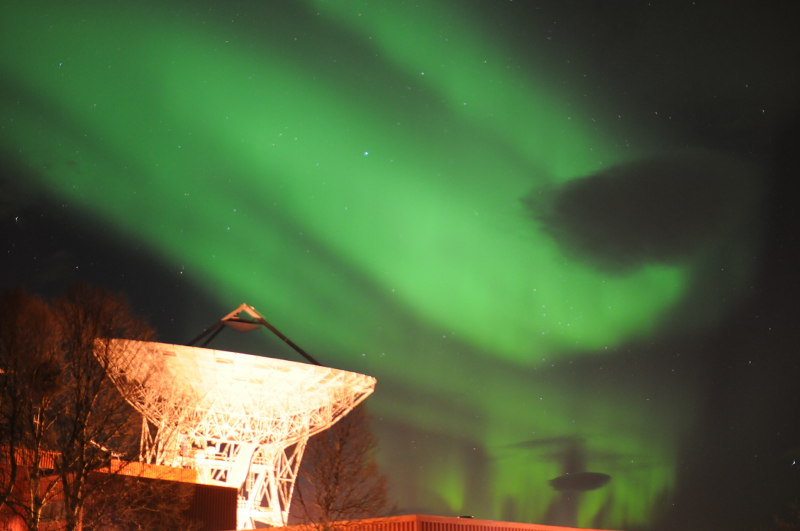
\includegraphics[height=\picsize]{uhf-tro-aurora.jpg}
% 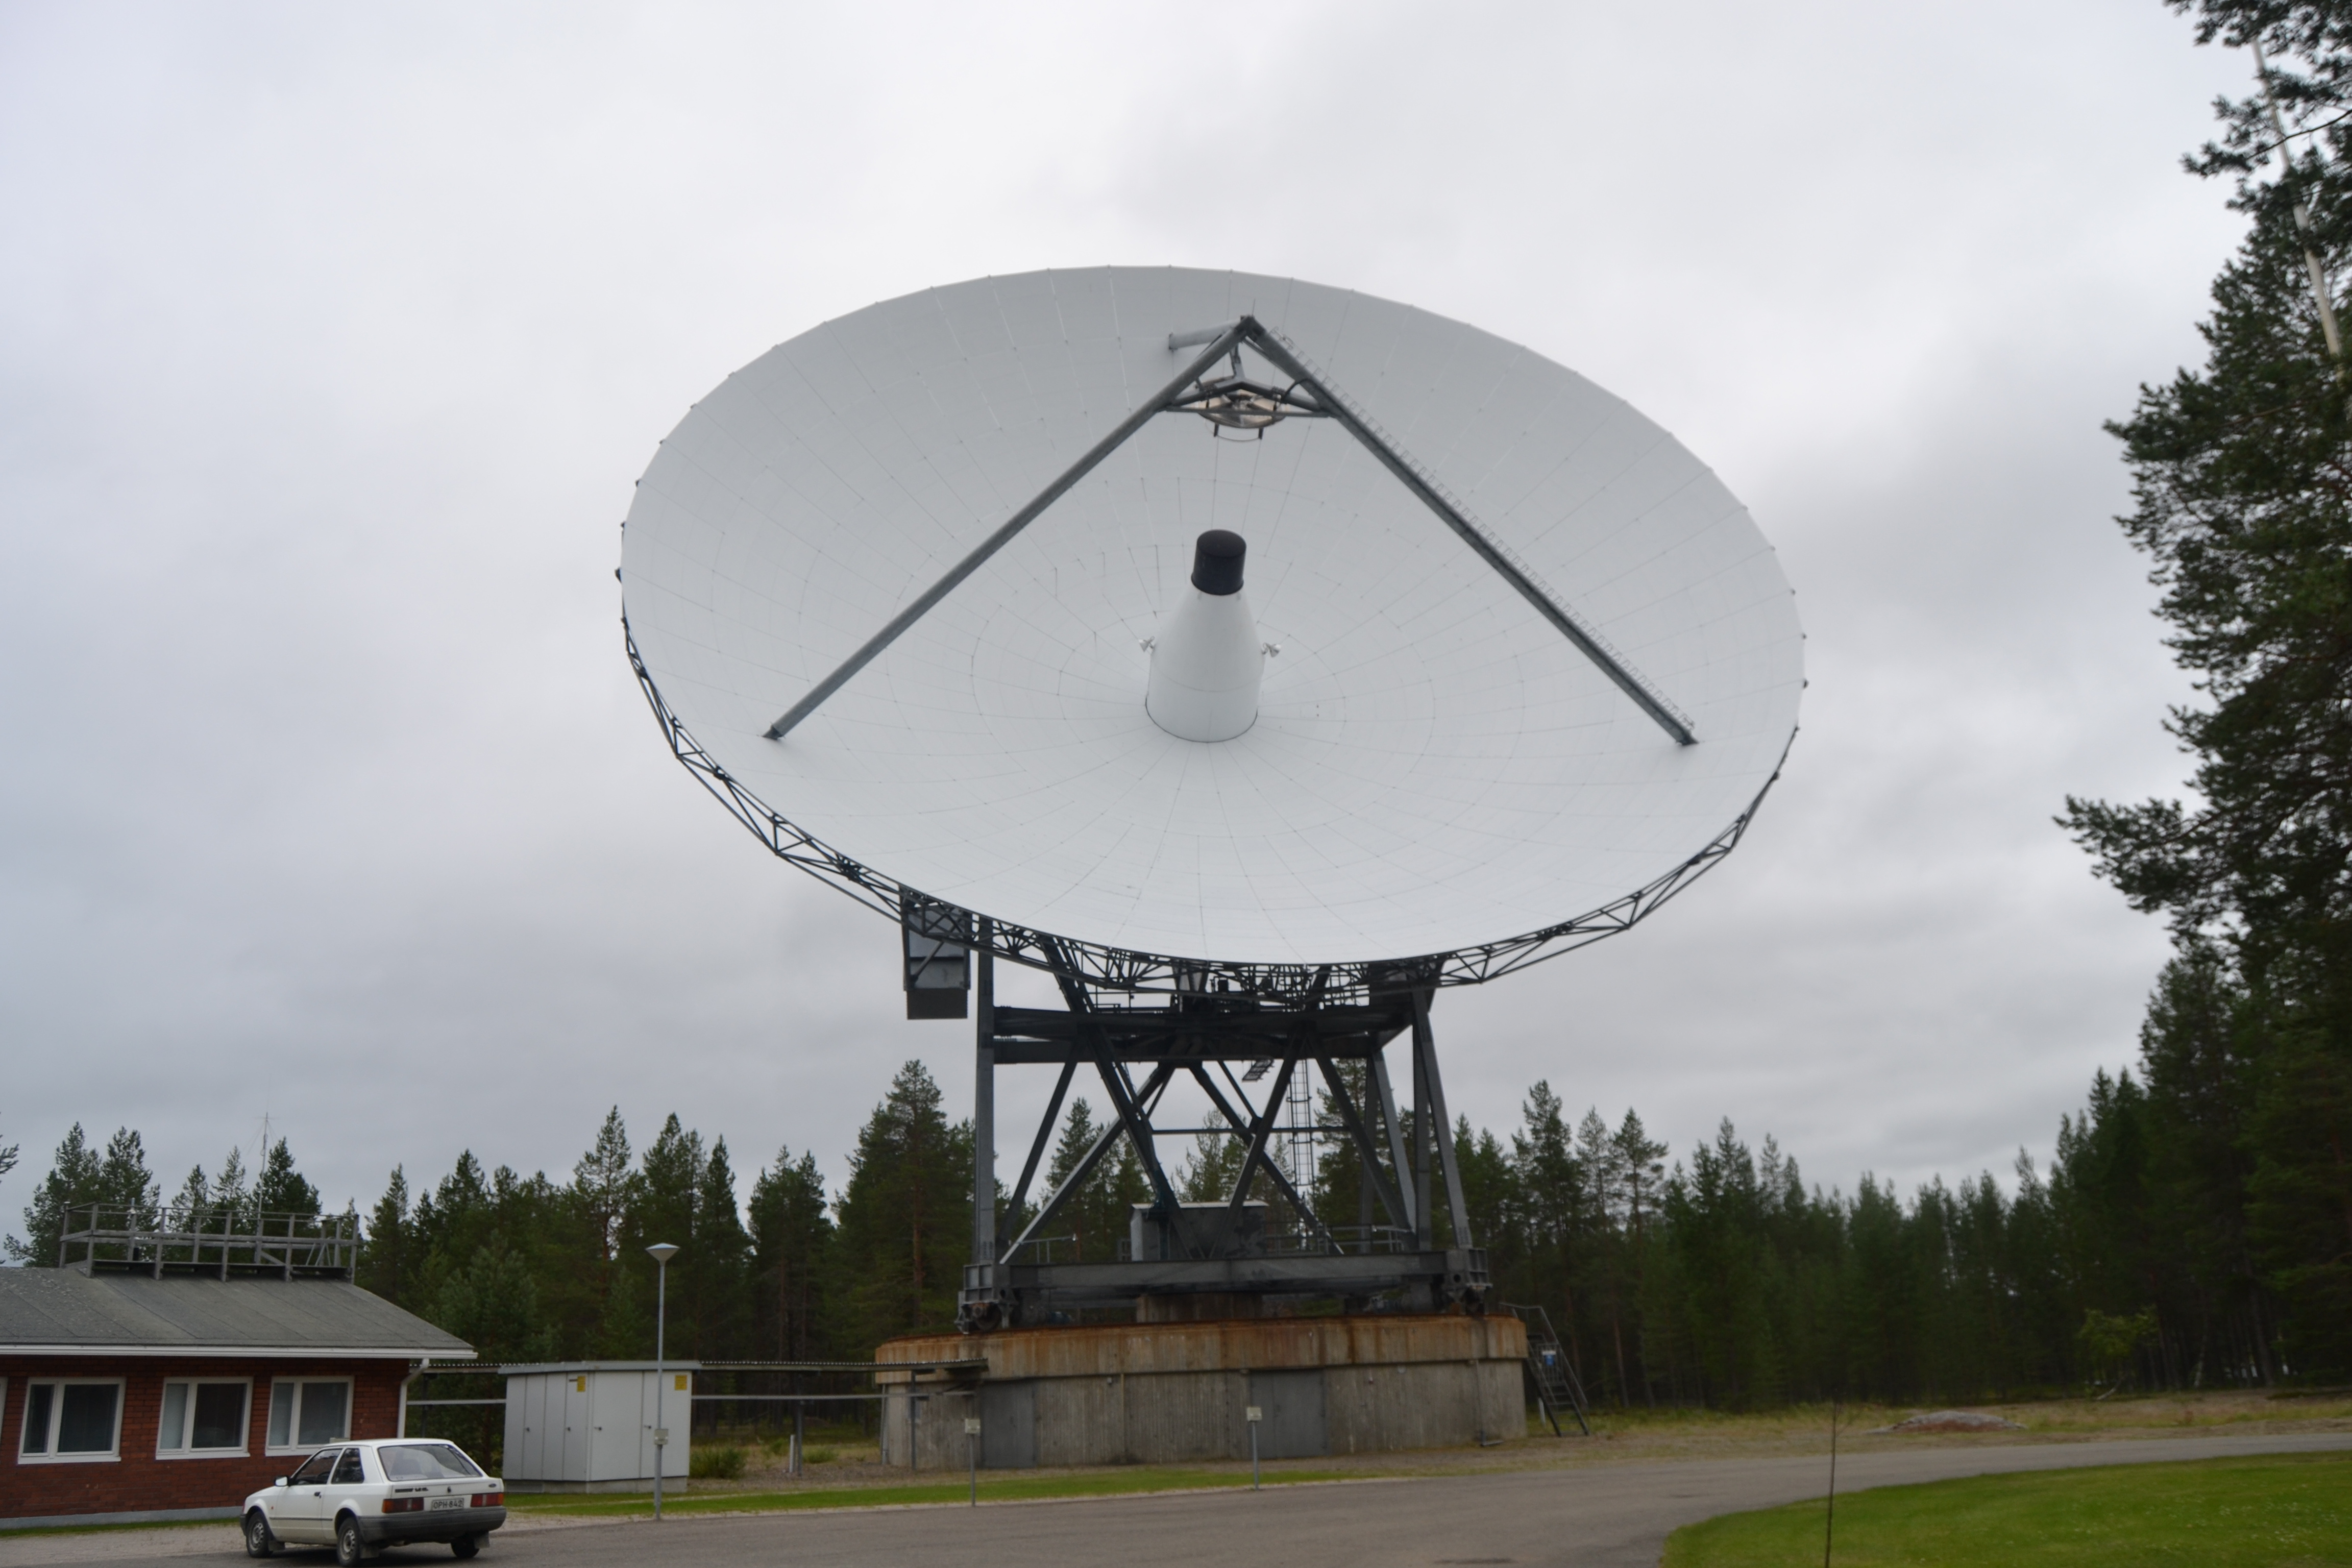
\includegraphics[height=\picsize]{EISCAT_Sodankyla_radar.jpg}
% 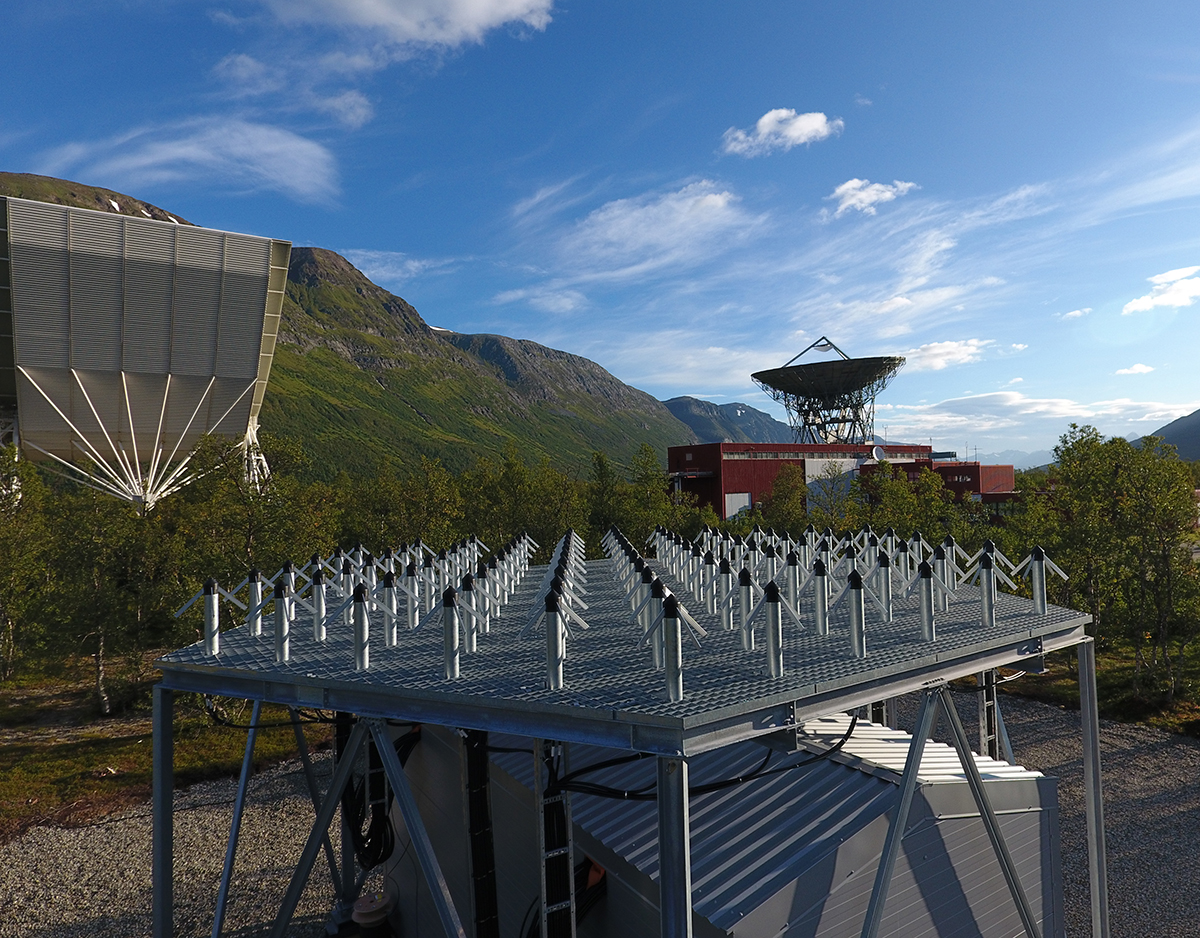
\includegraphics[height=\picsize,width=1.95in]{Tromso-eiscat3d.jpg}
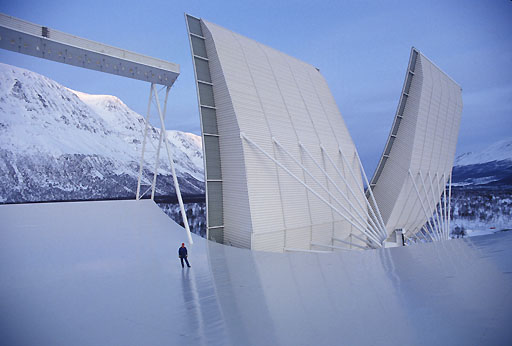
\includegraphics[height=\picsize,width=1.95in]{eiscat-vhf.jpg}

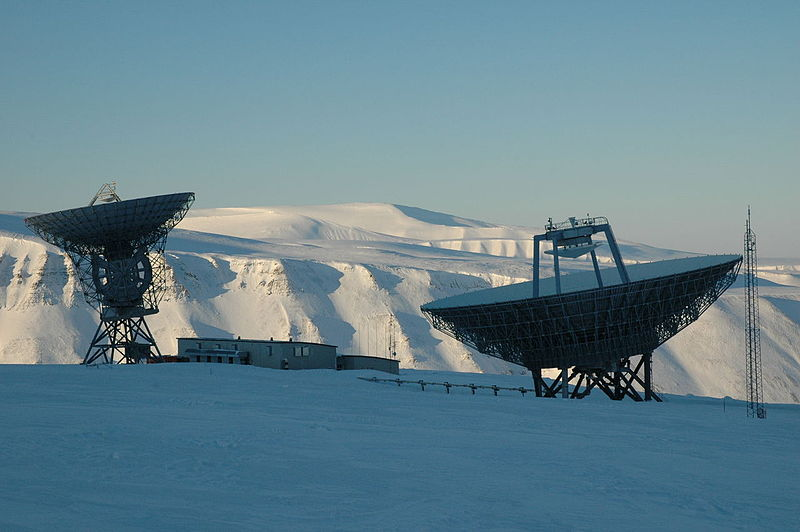
\includegraphics[height=\picsize]{EISCAT_Svalbard_Radar.jpg}
                \begin{minipage}{0.46\textwidth}{\colblack \scriptsize \it NASA via Wikimedia Commons, EISCAT}\end{minipage}
}
\end{center}
\vfill
    {\colblack {\bf E}uropean {\bf I}ncoherent {\bf Scat}ter Scientific Association ({\bf EISCAT})}
    {\small \url{https://www.eiscat.se/}}
\end{frame}

